\documentclass[12pt, addpoints]{exam/exam}

\usepackage{hyperref}
%\usepackage{mdframed}
\usepackage{graphicx, caption}	
%\usepackage{array, multicol, tabu}
\usepackage{amsmath, amsthm, amssymb}
\usepackage{comment}
\usepackage{enumitem}
\usepackage{url}
\usepackage{textcomp}
\newcommand{\vect}[1]{\mathbf{#1}}
\newcommand{\R}{\mathbb R}
\newcommand{\vstr}{\vspace{\stretch{1}}}
\everymath{\displaystyle}
\setlength{\parindent}{0pt}

\theoremstyle{plain}
\newtheorem{thm}{Theorem}
\newtheorem*{thm*}{Theorem}

%\printanswers
\pointformat{\bf(\thepoints)}
\pointpoints{pt}{pts}
\bonuspointformat{\bf(\thepoints)}
\bonuspointpoints{pt}{pts}

\coverfirstpageheader{\bf MATH 2574 (Calculus III) \\
		Spring 2017 \\
		}
		{}
		{{Name:} \underline{\hspace{40ex}} \\
		\vspace{0.5pc}
		Fri 10 Feb 2017}
\coverextraheadheight[2pc]{0in}
\coverfirstpagefooter{}{}{\Large Good luck!}
\coverrunningheader{}
	{Exam 1: Intro to Multidimensional Calculus}
	{}
\coverrunningheadrule	
\coverrunningfootrule
\coverrunningfooter{Wheeler}{Cal III Spring 2017}{p. \thepage\ (of \numpages)}

\firstpageheader{}
	{Exam 1: }
	{}
\firstpageheadrule
\firstpagefootrule
\firstpagefooter{Wheeler}{Cal III Spring 2017}{p. \thepage\ (of \numpages)}

\runningheadrule
\runningheader{}
	{Exam 1: Intro to Multidimensional Calculus}
	{}
\runningfootrule
\runningfooter{Wheeler}{Cal III Spring 2017}{p. \thepage\ (of \numpages)}

\title{\vspace{-8pc}
\vfill{\Huge
	\bf Exam 1: Intro to Multidimensional Calculus (\S 11.1-11.7,\ 12.1-12.2)} 
	}
%\author{}
\date{}

% % % % % % % % % % % % % % % % % % % %
\begin{document}

\begin{coverpages}
\maketitle
\thispagestyle{headandfoot}
\vspace{-4pc}
{\bf Exam Instructions:} You have 50 minutes to complete this exam.  Justification is required for all problems.  %Notation matters!  You will also be penalized for missing units and rounding errors.  
No electronic devices (phones, iDevices, computers, etc) except for a \textbf{basic scientific calculator}.  On story problems, round to one decimal place. If you finish early then you may leave, UNLESS there are less than 5 minutes of class left.  To prevent disruption, if you finish with less than 5 minutes of class remaining then please stay seated and quiet.

\begin{flushright}
In addition, please provide the following data:

\vspace{0.3in}
Drill Instructor: \underline{\hspace{40ex}}

\vspace{0.3in}
Drill Time: \underline{\hspace{40ex}}
\end{flushright}

\vfill
\textbf{Your signature below indicates that you have read this page and agree to follow the Academic Honesty Policies of the University of Arkansas.}  

\vspace{0.3in}
Signature: {\bf (1 pt)} \underline{\hspace{73ex}}

% % % % % % % % % %
\newpage

\begin{center}
\vspace*{\fill}
%\gradetable
\vspace*{\fill}
\end{center}
\end{coverpages}

% % % % % % % % % % % % % % % % % % % %
\begin{questions}
\thispagestyle{headandfoot}

% % % % %
\question %{\bf \S11.4 \#70, \S12.2 \#53}
Determine whether the following statements are true or false.  You must justify your answer.  
\begin{parts}
	\part[5] The domain of the function $u=f(w,x,y,z)$ is a region in $\R^4$.
	\vspace{11pc}
	
	\part[5] $(\vect u\times \vect v)\cdot \vect v=\vect 0$
	\vspace{11pc}
	
	\part[5]	The domain of the function $f(x,y)=1-|x-y|$ is $\{(x,y)\mid x\geq y\}$.
	\vspace{11pc}
	
	\part[5] All level curves of the plane $z=2x-3y$ are lines, except for when $z=0$.
	\vspace{11pc}
		
	%\bonuspart[] $\vect u\cdot (\vect v\times \vect w)=\vect w\cdot (\vect u\times \vect v)$
	%\vspace{10pc}
\end{parts}
\vstr 

\newpage
% % % % %
\question[18] %{\bf \S11.5 \#48}
Determine an equation of the line that is perpendicular to the lines 
\begin{align*}
\vect r(t) &= \langle -1+3t,3t,2t\rangle \\
\vect R(s) &= \langle -6+3s,-8+2s,-12+s\rangle 
\end{align*}
and passes through the point of intersection of the lines $\vect r$ and $\vect R$.

%\vstr

\newpage
% % % % %
\question %{\bf \S11.6 \#84}
Suppose $\vect u$ and $\vect v$ are differentiable functions at $t=0$ with $\vect u(0)=\langle 1,0,1\rangle,\ \vect u'(0)=\langle 7,0,1\rangle,\ \vect v(0)=\langle 0,1,1\rangle,\ \vect v'(0)=\langle 1,3,2\rangle$.  Evaluate the following expressions:
\begin{parts}
	\part[6] $\left.\frac{d}{dt}(\sin(t)\vect u(t))\right|_{t=0}$
	\vspace{20pc}
	
	\part[6] $\left.\frac{d}{dt}(\vect u\cdot \vect v)\right|_{t=0}$
	\vspace{20pc}
\end{parts}

%\vstr

\newpage
% % % % % 
\question %{\bf \S11.7 \#70,72}
A golfer stands 400 ft horizontally from the hole and 40 ft below the hole (see figure).  

\begin{center}
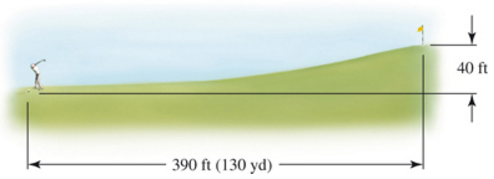
\includegraphics{exam1Golfer}
\end{center}

Suppose the ball is hit with an initial speed of 150 ft/s, at an angle of $\theta$ from the ground. 
\begin{parts}
\part[12] Find the acceleration $\vect a(t)$, velocity $\vect v(t)$, and position $\vect r(t)=\langle x(t),y(t)\rangle$ vectors for the trajectory of the ball.  The gravitational constant is $g=32$ ft/s$^2$.
\vspace{20pc}

\part[6] Write down a system of two equations to find the two unknowns: (1) time of flight and (2) $\theta$.  \textbf{Do not} solve the system.
\vspace{17pc}

\end{parts}
%\vstr 

\newpage
% % % % % 
\question[16] %{\bf \S 11.1 \#80}
A 100 kg box rests on a ramp with an incline of 30$^{\circ}$ to the floor (see figure).  Find the components of the force perpendicular to and parallel to the ramp.  (The vertical component of the force exerted by an object of mass $m$ is its weight, which is $mg$, where $g=9.8$ m/s$^2$ is the acceleration due to gravity.)

\begin{center}
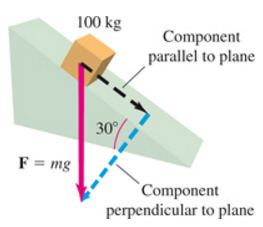
\includegraphics{exam1BoxOnARamp}
\end{center}

\vstr

\newpage
% % % % %
\question[15] %{\bf \S12.1 \#79} 
Match equations (a)-(f) with the surfaces (A)=(F).
\begin{enumerate}[label=(\alph*)]
	\item $y=|x|$
	\item $3x-4y-z=5$
	\item $y-z^2=0$
	\item $4x^2+\dfrac{y^2}{4}+z^2=1$
	\item $x^2+\dfrac{y^2}{9}=z^2$
	\item $x^2+\dfrac{y^2}{9}-z^2=1$
\end{enumerate}

\begin{center}
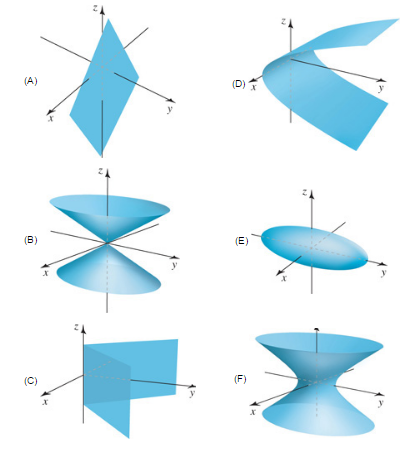
\includegraphics[scale=1.5]{exam1Surfaces}
\end{center}


 
%\begin{solutionbox}
\vspace
{2.5in}
%For both sums, $\Delta x=\frac{b-a}{n}=\frac{5-1}{8}=\left(\frac{1}{2}\right)$.
%\vspace{-1pc}
%\begin{align*}
%\text{LEFT:}\quad & \left(f(1)+f(1.5)+f(2)+f(2.5)+f(3)+f(3.5)+f(4)+f(4.5)\right)\left(\frac{1}{2}\right) \\
%	=& \left(0+2+3+2+2+1+0+2\right)\left(\frac{1}{2}\right)=\frac{12}{2}=\boxed{6} \\[0.2pc]
%\text{RIGHT:}\quad & \text{ LEFT}-f(1)\left(\frac{1}{2}\right)+f(5)\left(\frac{1}{2}\right) \\[0.2pc]
%		= & \ 6-\frac{0}{2}+\frac{3}{2} = \boxed{\frac{15}{2}}
%\end{align*}
%\end{solutionbox}
\vstr

%\newpage
% % % % %
%\bonusquestion {\bf EXTRA CREDIT!}  Evaluate the following sums using $\Sigma$-notation.
 
%\begin{parts}
% % % 
%\bonuspart[2] $1+3+5+7+\cdots +99$
%\begin{solutionbox}
%\vspace
%{1.5in}
%\vspace{-1.75pc}
%\begin{align*}
%\sum_{k=1}^{50}(2k-1) &= 2\sum_{k=1}^{50}k-\sum_{k=1}^{50}1 \\[0.2pc]
%	&= 2\left(\frac{50(50+1)}{2}\right)-1(50) \\[0.1pc]
%	&= 50(50)+50-50 = \boxed{2500}
%\end{align*}
%\end{solutionbox}
%\vstr

% % %
%\bonuspart[3] $4+9+14+\cdots +44$
%\begin{solutionbox}
%\vspace
%{1.75in}
%\vspace{-1.75pc}
%\begin{align*}
%\sum_{k=1}^9(5k-1) &= 5\sum_{k=1}^9k-\sum_{k=1}^91 \\[0.2pc]
%	&= 5\left(\frac{9(10)}{2}\right)-1(9) \\[0.1pc]
%	&= 45(9)-1(9) \\
%	&= 44(9)=4\cdot 11\cdot 9=4(99)=\boxed{396}
%\end{align*}
%\end{solutionbox}
%\vstr
% % %
%\bonuspart $3+8+13+\cdots +63$
%\vspace{1in}

% % %
%\part[] $\frac{1}{1\cdot 2}+\frac{1}{2\cdot 3}+\frac{1}{3\cdot 4}+\cdots+\frac{1}{49\cdot 50}$
%\vspace{0.5in}
%\end{parts}
%\vstr

\end{questions}

\end{document}